\newcommand{\figdir}{analysis/figures/}

\section{Evaluation}
\subsection{Techniques used in the evaluation}
All calculations in this section are done with scripts written in 
the \textit{python} programming language~\cite{python}, relaying in several 
packages:
\begin{itemize}
    \item
        \textit{matplotlib}~\cite{Hunter2007} for plotting,
    \item
        \textit{scipy}~\cite{scipy} for fitting, and 
    \item
        \textit{uncertainties}~\cite{uc} for error propagation.
\end{itemize}
The latter applies gaussian error propagation for correlated and uncorrelated variables. 
We will thus not explicitly write down the formulas for the error propagation 
for each quantity calculated but instead state the numerical result, only. 
We will, however make a quick remark on the use of covariance matrices in 
error propagation: Contrary to measured data, which in our case is usually 
expected to be uncorrelated, all fitted data yields variables that in general correlate. 
The propagation is then done as follows:
Let's assume we have random
variables $x_0,...,x_N$ which are correlated through the $N\times N$ Matrix $cov(x_i,x_j)$.
For a scalar function $f(x_0,...,x_N) \rightarrow \mathbb{R}$, the variance is estimated (linearly) by:
\begin{equation}
Var[f] = \sigma^2 = \sum_{i,j} \frac{\partial f}{\partial x_i} \frac{\partial f}{\partial x_j} cov(x_i,x_j) \,.
\end{equation} 
If instead, $\mathbf{f}$ is a vector field in $m$ dimensions, namely 
$\mathbf{f}(x_0,...,x_N) \rightarrow \mathbb{R}^m$, then the components of $\mathbf{f}$ 
are further correlated. We can write down the relation between the covariance matrices $V$ and $U$ of 
$\mathbf{x}$ and $\mathbf{f}$, respectively, in matrix relations:
\begin{equation}
    U = A V A^T
\end{equation}
where $A$ is the matrix defined by 
\begin{equation}
    A_{ij} = \left[ \frac{\partial f_i}{\partial x_j}\right]_{\mathbf{x} = \mathbf{\mu}}
\end{equation}
with expectation value $E[\mathbf{x}] = \mathbf{\mu}$.~\cite{cowan1998statistical}
In order to facilitate notation, the covariance matrices will in general be notated without 
specifying the units. If not specified explicitly, the units will correspond to those of the
variables: If $x_i, x_j$ have the units $[x_i], [x_j]$, respectively, 
then the entry of the covariance matrix has the unit $[x_i] * [x_j]$. 

\subsection{Lattice constant of sine grating}
Observing the intensity on the screen, we noticed that the beam was not 
diffracted in the plane $y = const.$ (where y denotes the horizontal direction). 
We thus notated the coordinates on the graph paper. The measured values 
are displayed in table \ref{tab:sine_distances}. The estimated error of 
$s_{xy} = 1$ mm in both directions mainly stems from the fact that the edge of the beam 
has only a limited sharpness. 
\renewcommand{\arraystretch}{1.5}
\begin{table}[htdp]
    \centering
    \begin{tabular}{|p{6.18cm}|p{3.82cm}|p{3.82cm}|}
        \hline
        \rowcolor{tabcolor}
        Maximum & $x$ / mm & $y$  / mm \\ \hline
        $0.$        & 3     & 3\\
        $1.$, left & 48    & -1\\
        $1.$, right  & -42   & 7\\
        \hline
    \end{tabular}
    \caption{
        Measurements of positions of maxima for the sine amplitude grating. 
        The error is estimated to be $s_{xy} := s_x = s_y = 1$ mm. 
        }
    \label{tab:sine_distances}
\end{table}
The distance $d_\mathrm{sin}$ between the zeroth and first maximum is calculated by taking half of 
the distance between the two first maxima:
\begin{align}
    d_\mathrm{sin}   &= \frac{1}{2} \sqrt{(x_l - x_r)^2 + (y_l - y_r)^2} = 45.1 \mathrm{mm} \\
    \begin{split}
        s_{d_\mathrm{sin}} &= \sqrt{\sum{
                \left(\frac{\partial d_\mathrm{sin}}{\partial x_i}\right)^2 s_{x_i}  + 
                \left(\frac{\partial d_\mathrm{sin}}{\partial y_i}\right)^2 s_{y_i} 
                }} \\
        &= \frac{s_{xy}}{\sqrt{2}} \\
        &= 0.7 \, \mathrm{mm}\, ,
    \end{split}
\end{align}
where $x_r, x_l$ and $y_r, y_l$ correspond to the coordinates of right and left 
maximum, respectively and $s_{d_\mathrm{sin}}$ denotes the error calculated by gaussian error propagation.
The distance between screen and grating was $l_\mathrm{sin} = (56 \pm 2)$ mm. By geometric construction, 
we can identify the angle $\theta$ between the lines connecting grating and the maxima 
of zeroth and first order on the screen, respectively. Using further the 
necessary condition for positive interference (see eqn \eqref{eq:inter_cond} in the theory section), 
we calculate the lattice constant $K_\mathrm{sin}$ for the sine grating:
\begin{align}
    \sin(\theta)&= \frac{d_\mathrm{sin}}{\sqrt{l_\mathrm{sin}^2 + d_\mathrm{sin}^2}} \\
    \sin(\theta)&= \frac{m\lambda}{K_\mathrm{sin}} \\
    \Rightarrow \qquad 
    K_\mathrm{sin}    &= m \lambda\sqrt{\left(\frac{l_\mathrm{sin}}{d_\mathrm{sin}}\right)^2 + 1} 
        = (1.01 \pm 0.02) \, \mu\mathrm{m} \\
\end{align}
Although no nominal value is stated, the measured value suggests, that the grating has been 
constructed to a nominal value of $K_\mathrm{sin, nom} = 1$ $\mu$m. 

\subsection{Calibration}
For all further measurements, we needed to calibrate the setup and use the gauge gratings 
to establish the relationship between the signal observed on the oscilloscope and the 
actual distance between the peaks which would be observed on a screen at the position of diode 1. 
For this part, we set the lenses such that the beam would be widened and collimated. We tested the collimation 
with the graph paper. The measured distances can be seen in the handwritten records, see appendix \ref{sec:records}.
The small focal length of lens 3 ($f_3 = 300$ mm) made it impossible to focus the beam exactly onto diode 1. We 
chose the closest position allowed by the setup, such the lens would not interfere with the second beam. 

We measured the peaks with the amplitude grating two times, since we noticed a difference when turning the grating. 
Both measurements are plotted in figure \ref{fig:calibrate_peaks}. 
We searched for the times at the maxima numerically, taking the center value in case of a plateau. 
The results are plotted as dotted lines, the numbers are given in table \ref{tab:gauge_peaks}. 
The error was estimated somewhat bigger then the calculated standard deviation (in almost 
    all cases, $s_{\overline{t_\mathrm{max, calculated}}}  = 0.004$ ms), which has little meaning, 
since we only took two measurements. The estimated errors are then further propagated for the fits. 

\renewcommand{\arraystretch}{1.5}
\begin{table}[htdp]
    \centering
    \begin{tabular}{|p{3cm}|p{2cm}|p{2cm}|p{2cm}|}
        \hline
        \rowcolor{tabcolor}
        Maximum & $t_1$ / ms & $t_2$  / ms & $\overline{t_\mathrm{max}}$ / ms \\ \hline
        $3.$, left  & 0.204     & 0.211 & 0.207 \\
        $2.$, left  & 0.298     & 0.306 & 0.302 \\
        $1.$, left  & 0.393     & 0.400 & 0.397 \\
        $0.$,       & 0.489     & 0.496 & 0.492 \\
        $1.$, right & 0.585     & 0.591 & 0.588 \\
        $2.$, right & 0.682     & 0.686 & 0.684 \\
        \hline
    \end{tabular}
    \caption{
        Peaks for the calibration grating. We estimate the error on each 
        value of $\overline{t_\mathrm{max}}$ with 
        $s_{\overline{t_\mathrm{max}}} = 0.01$ ms for all maxima except the 
        very small peak for $m = 2$ on the right side ($s = 0.04$).
        }
    \label{tab:calibrate_peaks}
\end{table}
\begin{figure}[htpb]
    \centering
    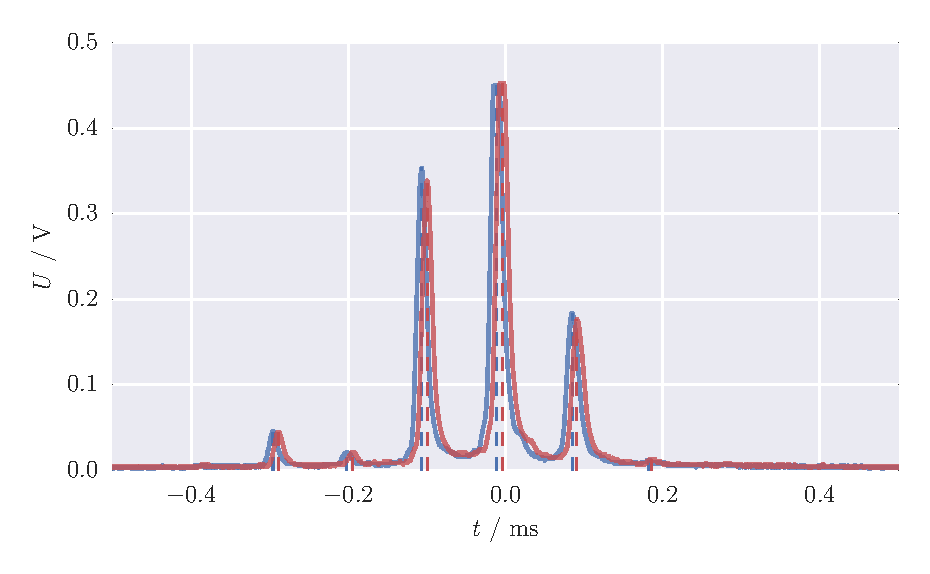
\includegraphics[width=1.0\linewidth]{figures/calibrate_peaks}
    \caption{
        Measured signal for the gauge gratings, each corresponding to a different orientation of the 
        grating. The maxima are found numerically, taking the central value in case of a plateau. 
        The is a clear offset of the maxima corresponding to the same order. For further calculations, 
        we take the mean value of the two. 
        }
     \label{fig:calibrate_peaks}
\end{figure}

From the maxima, we could calculate the linear correspondence $\theta(t)$, 
which is derived by \ref{eq:N_lines_interference}:
\begin{equation}
    \theta(m) = \arcsin\left(\frac{m \lambda}{K}\right)
\end{equation}
Since the mirror rotates with constant angular speed $\omega_1$, we can 
also write $\theta(t)$. By correctly identifying the maxima, and using the 
known lattice constant $K_\mathrm{gauge}$ of the gauge grating, we can perform a linear fit.
The result is plotted in figure \ref{fig:calibrate_fit}. The values and the corresponding 
covariance matrix are: 
\begin{align}
	\omega &= 0.0663 \\
	\theta_0 &= 0.0005 \\
	\mathrm{cov} &=
	\begin{pmatrix}
		2.0\mathrm{e}-07 &-6.1\mathrm{e}-09 \\
		-6.1\mathrm{e}-09 &6.0\mathrm{e}-09 \\
	\end{pmatrix} 
\end{align}
The standard deviation $\sigma_\omega$ of the relevant parameter $\omega$ is only about 
$\sigma_\omega / \omega = sqrt(2.0 * 10^{-7}) / 0.0663 \approx 0.7 \%$. 
This small error is linked to the constant rotational speed 
one could expect of the motor. The correlation of $\omega$ to $\theta_0$ is of one magnitude smaller 
than the variance - the effect could thus be neglected in the further calculations (although we keep 
    on using the correlated variables).

\begin{figure}[htpb]
    \centering
    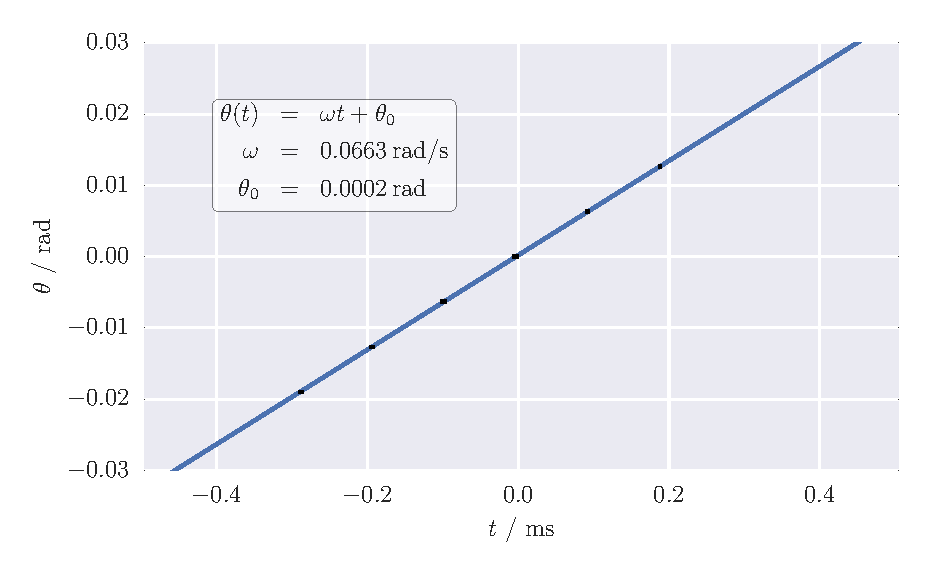
\includegraphics[width=1.0\linewidth]{figures/calibrate_fit}
    \caption{
        Fit of the angles identified for the gauge grating with known 
        lattice constant of $K = 10,000$ lines/m. The errors on the time corresponds to the
        shift observed when turning the grating around. The fit is drawn with the errors obtained 
        by error propagation using the corresponding covariance matrix.
        }
    \label{fig:calibrate_fit}
\end{figure}

\subsection{Lattice constant and resolution for five gratings}
Using $\theta(t)$, we can calculate the lattice constants for the five amplitude gratings. 
For that, we find the times corresponding to the $m$th maximum numerically. The width 
of the peaks is approximately equal at half maximum, such that we do not put weights 
on each maximum. We also neglect to fit gaussians on each peak. An application of such methods 
for this measurement does not increase the precision of the measurement to a appreciable degree, 
as the peaks in the measured data are already quite symmetric and the applied simpler method yields 
good results, at least in comparison with other errors. 
Plots of the measured data and the maxima can be found in the appendix, see 
\ref{fig:gratings_maxima}. 

We again apply the formula \ref{eq:N_lines_interference}. Since we use numerical computation, 
there is no need to do the first order approximation of the sine. The lattice constants are thus 
found by
\begin{equation}
    K_i = \frac{m\lambda}{\sin(\theta)}\, .
\end{equation}
One observes from the plotted data that only a finite number of maxima is seen and, more important, 
that some maxima of lower order than the highest maximum observable are not visible, either. 
Thus, assigning the maxima has to be done by hand, already assuming the almost equal distances between the 
maxima. In order to calculate the angle $\theta$, we translated the time $t_\mathrm{osci} \rightarrow t$ 
such that $t = 0$. 
This had to be done, as the oscilloscope did not save the time with respect to the trigger 
but set $t = 0$ to the first data point. 

\begin{table}[htdp]
    \centering
	\begin{tabular}{|p{3.82cm}|p{6.18cm}|p{3.82cm}|}
		\hline
		\rowcolor{tabcolor}
		Grating & Orders visible & $\overline{K_i}$ / ($\mu$m)  \\ \hline
		$1$  & $-4, -3, -2, -1, 0, 1, 2, 3, 4$  & $ 126.2 \pm 1.2$ \\
		$2$  & $-3, -2, -1, 0, 1, 2$            & $ 34.3 \pm 1.3$ \\
		$3$  & $-5, -4, -2, -1, 0, 1, 2, 4, 5$  & $ 100.6 \pm 4.4$ \\
		$4$  & $-5, -3, -1, 0, 1, 3, 5$         & $ 101.0 \pm 1.5$ \\
		$5$  & $-2, -1, 0, 1, 2$                & $ 50.9 \pm 1.3$ \\
		\hline
	\end{tabular}
    \caption{
        Calculated lattice constants of amplitude gratings one to five. 
        The orders $m$ have to be assigned by hand, as for grating 3 and 4 some 
        orders in between are missing. The error is the standard deviation of 
        the weighted mean.
        }
    \label{tab:gratings_K}
\end{table}

The resolution of the gratings can be calculated as described in the theory section, 
see equation \eqref{eq:resolution}.
The diameter $\phi$ of the laser in this experiment was measured with a slide gauge. 
\begin{equation}
    \phi = (2.9 \pm 0.5) \, \mathrm{mm}
\end{equation}
We approximate the number $N$ of lines illuminated by
\begin{equation}
    N = \phi / K
\end{equation}
with lattice constant $K$. The number of lines observed at full illumination and the
resulting resolution $a$ using the previously estimated lattice constants $\overline{K_i}$
are displayed in table \ref{tab:gratings_resolution}. During the experiment, the resolution was 
limited not only to the natural resolution of the gratings with the applied beam, but 
also due to the fact, that the trigger also passed diode 1, such that an observable peak
might have been overlapped by this signal. We restricted ourselves to use only those
directly visible, however. 

\begin{table}[htdp]
    \centering
    	\begin{tabular}{|p{2cm}|p{3.82cm}|p{3.82cm}|p{3.82cm}|}
		\hline
		\rowcolor{tabcolor}
		Grating & $n$ orders visible & $N$ lines illuminated & resolution $a$ \\ \hline
		$1$  & $10$ & $23.1 \pm 4.1$ & $ 230 \pm 40 $ \\
		$2$  & $6$ & $84.8 \pm 14.8$ & $ 508 \pm 88 $ \\
		$3$  & $10$ & $28.7 \pm 5.0$ & $ 287 \pm 50 $ \\
		$4$  & $9$ & $28.7 \pm 5.0$ & $ 258 \pm 44 $ \\
		$5$  & $6$ & $57.1 \pm 10.1$ & $ 342 \pm 60 $ \\
		\hline
	\end{tabular}

    \caption{
        Resolutions of five gratings for largest illumination possible 
        in the experiment (diameter of laser $\phi = 2.9 \pm 0.5$). 
        We used the lattice constants calculated before, \ref{tab:gratings_K}. 
        }
    \label{tab:gratings_resolution}
\end{table}

\subsection{Aperture function}
In this section we calculate the aperture function of grating 1 from the intensity 
of the maxima observed. 
